\documentclass{article}
\usepackage[a4paper, margin=3mm, landscape]{geometry}
\usepackage{multicol}
\usepackage{xcolor}
\usepackage{enumitem}
\usepackage{amsmath}
\usepackage{amsfonts}
\usepackage{listings}
\usepackage{soul}
\usepackage{graphicx}

\pdfinfo{
    /Title (CS2109S.pdf)
    /Creator (TeX)
    /Producer (pdfTeX 1.40.0)
    /Author (Jason Qiu)
    /Subject (CS2109S)
    /Keywords (CS2109S, nus, cheatsheet, pdf)
}

\graphicspath{ {./img/} }

\pagestyle{empty}
\setcounter{secnumdepth}{0}
\setlength{\columnseprule}{0.25pt}

% Redefine section commands to use less space
\makeatletter
\renewcommand{\section}{\@startsection{section}{1}{0mm}%
    {-1ex plus -.5ex minus -.2ex}%
    {0.5ex plus .2ex}%x
{\normalfont\large\bfseries}}
\renewcommand{\subsection}{\@startsection{subsection}{2}{0mm}%
    {-1explus -.5ex minus -.2ex}%
    {0.5ex plus .2ex}%
{\normalfont\normalsize\bfseries}}
\renewcommand{\subsubsection}{\@startsection{subsubsection}{3}{0mm}%
    {-1ex plus -.5ex minus -.2ex}%
    {1ex plus .2ex}%
{\normalfont\small\bfseries}}%
\makeatother

% Adjust spacing for all itemize/enumerate
\setlength{\leftmargini}{0.5cm}
\setlength{\leftmarginii}{0.5cm}
\setlist[itemize,1]{leftmargin=2mm,labelindent=1mm,labelsep=1mm}
\setlist[itemize,2]{leftmargin=2mm,labelindent=1mm,labelsep=1mm,label=$\bullet$}

% Font
\renewcommand{\familydefault}{\sfdefault}

% Define colors for math formulas
\definecolor{myblue}{cmyk}{1,.72,0,.38}
\everymath\expandafter{\the\everymath \color{myblue}}

% Custom command for keywords
\definecolor{highlight}{RGB}{251,243,218}
\newcommand{\keyword}[2][]{\sethlcolor{highlight}\hl{\textbf{#2}} #1 - }
\newcommand{\ilkeyword}[1]{\sethlcolor{highlight}\hl{\textbf{#1}}}

% Define colors and style for code
\definecolor{codegreen}{rgb}{0,0.6,0}
\definecolor{codegray}{rgb}{0.5,0.5,0.5}
\definecolor{codered}{HTML}{CC241D}
\definecolor{backcolor}{rgb}{0.95,0.95,0.95}
\lstdefinestyle{codestyle}{
    backgroundcolor = \color{backcolor},
    commentstyle = \color{codegray},
    keywordstyle = \color{codered},
    stringstyle = \color{codegreen},
    basicstyle = \ttfamily,
    breakatwhitespace = false,
    showstringspaces = false,
    breaklines = true,
    showtabs = false,
    tabsize = 2
}
\lstset{style = codestyle}

% -----------------------------------------------------------------------
\begin{document}
\begin{multicols*}{3}
\footnotesize

% Title box
\begin{center}
    \fbox{
        \parbox{0.8\linewidth}{
            \centering \textcolor{black}{
                {\Large\textbf{CS2109S}} \\
                \normalsize{AY22/23 Sem 2}} \\
                {\footnotesize \textcolor{gray}{github.com/jasonqiu212}}
        }
    }
\end{center}

\section{01. Introduction}

\begin{itemize}
    \item \keyword{Agent}{Anything that can perceive its environment through sensors and acting upon that env. through actuators}
    \item \keyword{Agent Function}{Maps from percept histories to actions}
    \item \keyword{Rational Agent}{Chooses an action that is expected to maximize its performance measure, given by percept sequence and built-in knowledge}
    \item \keyword{Autonomous Agent}{If behavior is determined by its own expereince}
\end{itemize}

\subsection{Performance Measure of Function}

\begin{itemize}
    \item Motivation: For an agent to do the right thing, need a measure of goodness
    \item Performance vs. Cost
\end{itemize}


\begin{enumerate}
    \item Best for whom?
    \item What are we optimizing?
    \item What information is available?
    \item What are the side effects and costs?
\end{enumerate}

\subsection{Defining the Problem: PEAS}

\begin{enumerate}
    \item Performance measure
    \item Environment
    \item Actuators
    \item Sensors
\end{enumerate}

\subsection{Characterizing the Environment}

\begin{enumerate}
    \item \keyword{Fully observable}{(vs. Partially) Agent's sensors can access complete state of env. all the time}
    \item \keyword{Deterministic}{(vs. Stochastic) Next state of env. is determined by \textbf{current state} and \textbf{action executed by agent}}
    \begin{itemize}
        \item \keyword{Strategic}{If env. is deterministic except for actions of other agents}
    \end{itemize}
    \item \keyword{Episodic}{(vs. Sequential) Agent's experience is divided into atomic \textbf{episodes}, where each episode includes perceiving and an action, and \textbf{action depends on episode} itself}
    \item \keyword{Static}{(vs. Dynamic) Env. is unchanged while agent is deciding}
    \begin{itemize}
        \item \keyword{Semi}{Time does not affect env., but affects performance score}
    \end{itemize}
    \item \keyword{Discrete}{(vs. Continuous) Discrete num. of percepts and actions}
    \item \keyword{Single Agent}{(vs. Multi-agent) Agent operating by itself in an env.}
\end{enumerate}

\subsection{Implementing Agents (in ascending complexity)}

\begin{enumerate}
    \item \keyword{Simple Reflex Agents}{Fixed conditional rules}
    \item \keyword{Model-based Reflex Agents}{Stores percept history to make decisions about internal model of world with conditional rules. Eg. Roomba}
    \item \keyword{Goal-based Agents}{Keep in mind a goal and action aims to achieve it}
    \item \keyword{Utility-based Agents}{Find best way to achieve goal}
    \item \keyword{Learning Agents}{Learn from previous experiences}
\end{enumerate}

\subsection{Exploitation vs. Exploration}

\begin{itemize}
    \item \keyword{Exploitation}{Maximize expected utility using current knowledge of world}
    \item \keyword{Exploration}{Learn more about the world to improve future gains. May not always maximize performance measure.}
\end{itemize}

\section{02. Uninformed Search}

\begin{itemize}
    \item Deterministic, fully observable
    \item \keyword{Tree Search}{Can revisit nodes}
    \item \keyword{Graph Search}{Tracks visited (Tree Search + Memoization)}
    \item \keyword{Uninformed Search}{Uses only information available in problem definition}
\end{itemize}

\subsection{Formulating the Problem}

\begin{enumerate}
    \item How to represent state in problem?
    \item Initial state
    \item Actions: Successor function
    \item Goal test
    \item Path cost
\end{enumerate}

\begin{itemize}
    \item \keyword{Abstraction Function}{Maps abstracted representation to real world state}
    \item \keyword{Representation Invariant}{$I(c) = \textbf{True} \rightarrow \exists a \textbf{ s.t. } AF(c) = a$}
\end{itemize}

\subsection{Breadth-first Search}

\begin{itemize}
    \item Idea: Expand shallowest unexpanded node using \textbf{queue}
    \item Given: $b$: Branching factor and $d$: Depth of optimal solution
    \item Complete: Yes (if tree is finite)
    \item Time: $O(b^{d+1})$
    \item Space: $O(b^d)$
    \item Optimal: Yes (if cost = 1)
    \item BFS is Uniform-cost Search with same cost
\end{itemize}

\subsection{Uniform-cost Search}

\begin{itemize}
    \item Idea: Expand least-cost unexpanded node using \textbf{priority queue} (Dijkstra's)
    \item Given: $C^*$: Cost of optimal solution
    \item Complete: Yes (if step cost $\geq \epsilon$ where $\epsilon \geq 0$)
    \item Time: $O(b^{(C^* / \epsilon)})$ ($C^* / \epsilon$ is approx. number of layers)
    \item Space: $O(b^{(C^* / \epsilon)})$
    \item Optimal: Yes
\end{itemize}

\subsection{Depth-first Search}

\begin{itemize}
    \item Idea: Expand deepest unexpanded node using \textbf{stack}
    \item Given: $m$: Maximum depth of tree
    \item Complete: No (fails with infinite depth or loops)
    \item Time: $O(b^m)$
    \item Space: $O(bm)$ (better than BFS)
    \item Optimal: No
\end{itemize}

\subsection{Depth-limited Search}

\begin{itemize}
    \item Motivation: How to handle infinite depth for DFS?
    \item Idea: DFS with depth limit $I$ where nodes at depth $I$ have no children
    \item Time: $b^0 + b^1 + ... + b^{(d - 1)} + b^d = O(b^d)$
\end{itemize}

\subsection{Iterative Deepening Search}

\begin{itemize}
    \item Motivation: How to determine depth limit? We don't.
    \item Idea: Try different depths for depth-limited search
    \begin{itemize}
        \item BFS pretending to be DFS to save space
    \end{itemize}
    \item Complete: Yes
    \item Time: $(d + 1)b^0 + db^1 + ... + b^d = O(b^d)$ (More overhead than DLS)
    \item Space: $O(bd)$
\end{itemize}

\subsection{Summary}

\begin{tabular}{ |c|c|c|c|c|c| }
    \hline
    & \textbf{BFS} & \textbf{Uniform Cost} & \textbf{DFS} & \textbf{DLS} & \textbf{IDS} \\
    \hline
    \textbf{Complete} & Yes & Yes & No & No & Yes \\
    \hline
    \textbf{Time} & $O(b^d)$ & $O(b^{C^* / \epsilon})$ & $O(b^m)$ & $O(b^l)$ & $O(b^d)$ \\
    \hline
    \textbf{Space} & $O(b^d)$ & $O(b^{C^* / \epsilon})$ & $O(bm)$ & $O(bl)$ & $O(bd)$ \\
    \hline
    \textbf{Optimal} & Yes & Yes & No & No & No \\
    \hline
\end{tabular}

\subsection{Bidirectional Search}

\begin{itemize}
    \item Idea: Search both forwards from initial state and backwards from goal state. Stop when searches meet.
    \item Time: $O(2 b^{d/2})$
    \item Operators must be reversible
    \item Can have many goal states
    \item How to check if node intersects with other half?
\end{itemize}

\section{03. Informed Search}

\subsection{Heuristic}

\begin{itemize}
    \item \keyword{Heuristic}{Estimated cost from $n$ to goal}
    \item \keyword{Admissible}{$h(n)$ is admissible if, for every node $n$, $h(n) \leq h^*(n)$ where $h^*$ is the true cost}
    \begin{itemize}
        \item if $h$ is admissible, then A* using tree search is optimal
    \end{itemize}
    \item \keyword{Consistent}{$h(n)$ is consistent if, for every node $n$ and every successor $n'$ of $n$ generated by action $a$, $h(n) \leq c(n, a, n') + h(n')$}
    \begin{itemize}
        \item Triangle inequality
        \item If $h$ is consistent, $f(n)$ is non-decreasing along any path ($f(n') \geq f(n)$)
        \item If $h$ is consistent, then $h$ is admissible
        \item if $h$ is admissible, then A* using graph search is optimal
    \end{itemize}
\end{itemize}

\subsubsection{Dominance}

\begin{itemize}
    \item If $h_2 (n) \geq h_1 (n)$ for all $n$, then $h_2$ \ilkeyword{dominates} $h_1$
    \item If $h_2$ \ilkeyword{dominates} $h_1$ and both are admissible, then $h_2$ is better for search
\end{itemize}

\subsubsection{How to invent admissible heuristic?}

\begin{itemize}
    \item Set fewer restrictions on actions
    \item E.g. Number of misplaced tiles, Total manhattan distance
\end{itemize}

\subsection{Best-first Search}

\begin{itemize}
    \item Idea: Expand most desirable node using priority queue
    \item Evaluation Function: $f(n) = h(n)$
    \item Complete: No. Possible to be stuck in loop
    \item Time and space: $O(b^m)$
    \item Optimal: No
\end{itemize}

\subsection{A* Search}

\begin{itemize}
    \item Idea: Take note of cost so far and heuristic
    \item Evaluation Function: $f(n) = g(n) + h(n)$ where $g(n)$ is cost to reach $n$ 
    \item Complete: Yes, unless non-increasing, since cost is factored in
    \item Time and space: Same as BFS
    \item Yes, depending on the heuristic
\end{itemize}

\subsection{Iterative Deepening A* Search (IDA*)}

\begin{itemize}
    \item Motivation: How can we save space?
    \item Idea: Have a cutoff for $f$ and remember the best $f$ that exceeds cutoff
    \begin{itemize}
        \item Similar to IDS. Linear space complexity.
    \end{itemize}
    \item Optimal and complete
\end{itemize}

\subsection{Simplified Memory A* Search (SMA*)}

\begin{itemize}
    \item Motivation: How can we save space?
    \item Idea: Do normal A*. If memory is full, drop node with worst $f$.
    \item Lose completeness
\end{itemize}

\section{04. Adversial Search}

\begin{itemize}
    \item Assumption: Opponents reacts rationally
    \item Needs:
    \begin{itemize}
        \item Initial state
        \item Successor function
        \item Terminal test
        \item Utility function: Measures how good the move is for a player
    \end{itemize}
\end{itemize}

\subsection{Minimax}

\begin{itemize}
    \item Idea: Choose move that yields highest minimax value
\end{itemize}

\section{05. Introduction to Machine Learning}

\begin{itemize}
    \item A machine learns if it improves performance P on task T based on experience E. Where T must be fixed, P must be measurable, E must exist
\end{itemize}

\subsubsection{Types of Feedback}

\begin{itemize}
    \item \keyword{Supervised}{Correct answer given for each example}
    \begin{itemize}
        \item \keyword{Regression}{Predict results within continuous output}
        \item \keyword{Classification}{Predict results in discrete output}
    \end{itemize}
    \item \keyword{Unsupervised}{No answers given}
    \item \keyword{Weakly supervised}{Answer given, but not precise}
    \item \keyword{Reinforcement}{Occasional rewards given}
\end{itemize}

\subsection{Decision Trees}

\begin{itemize}
    \item DT can express any function of input attributes, if data is consistent
    \item Goal: Make DT \textbf{compact}. How?
\end{itemize}

\subsubsection{Information Theory}

\begin{itemize}
    \item Idea: Choose attribute that splits examples into subsets that are ideally 'all positive' or 'all negative'
    \item \keyword{Entropy}{Measure of randomness in set of data}
\end{itemize}

\[I(P(v_1), ..., P(v_n)) = - \sum^{n}_{i = 1} P(v_i) \log_{2} P(v_i)\]

\begin{itemize}
    \item For data with $p$ positive examples and $n$ negative examples:
\end{itemize}

\[I(\frac{p}{p + n}, \frac{n}{p + n}) = - \frac{p}{p + n} \log_{2} \frac{p}{p + n} - \frac{n}{p + n} \log_{2} \frac{n}{p + n}\]

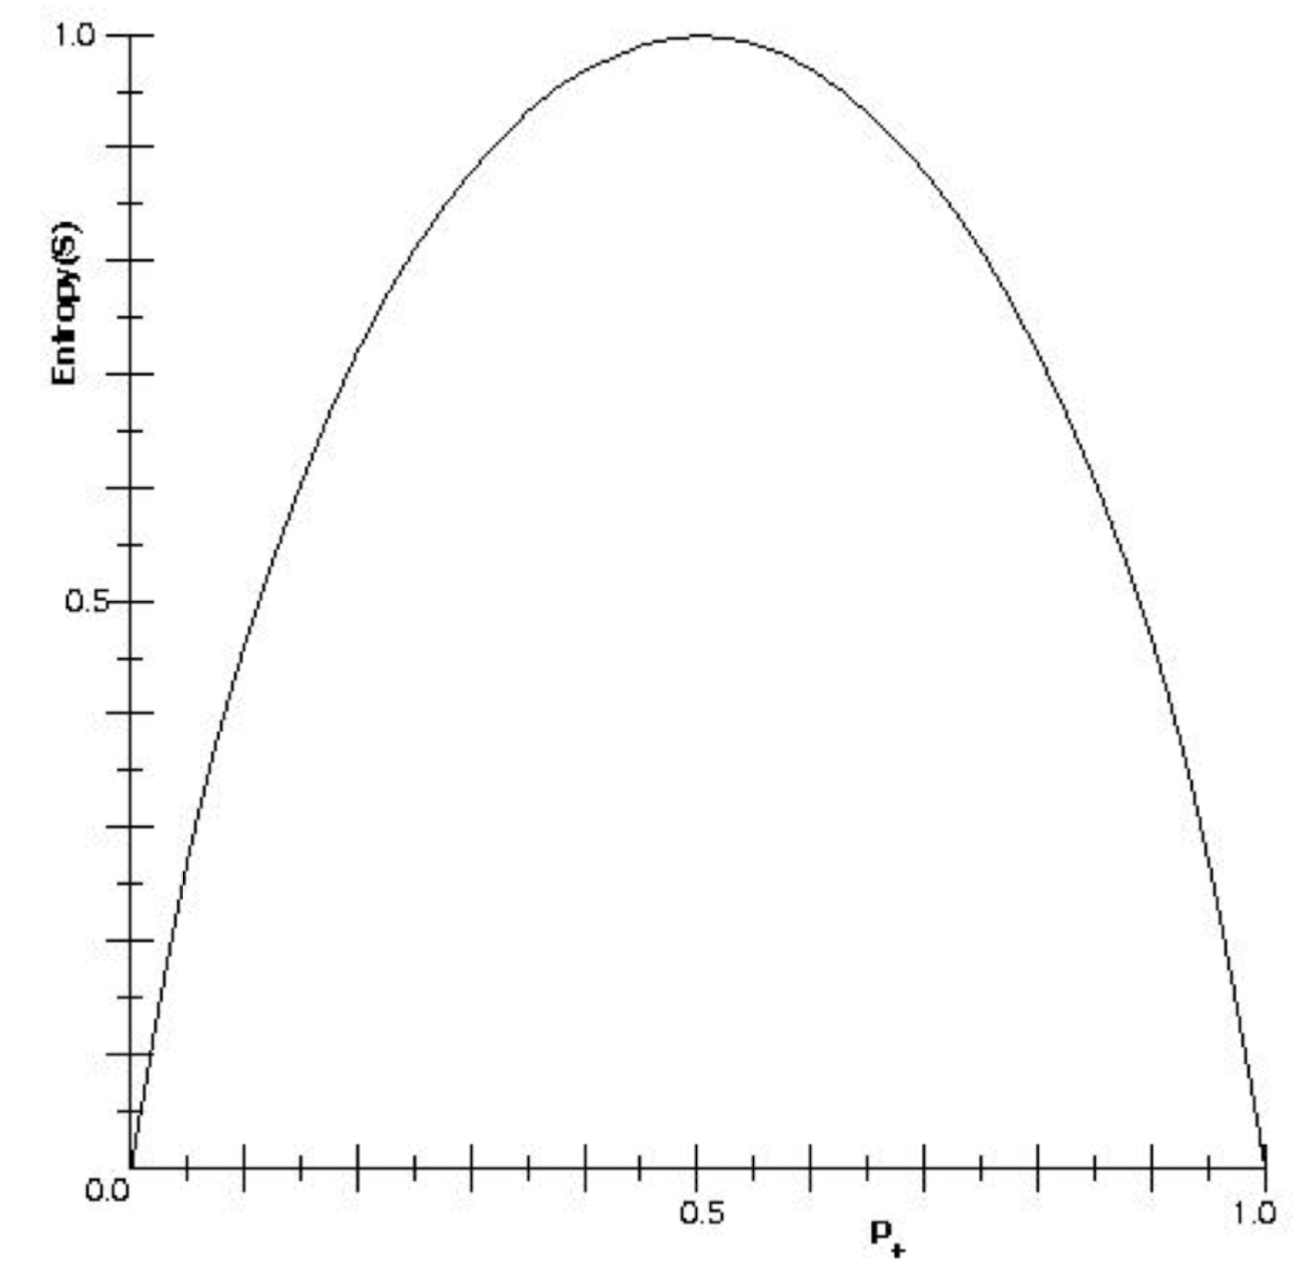
\includegraphics[scale=0.15]{entropy}

\begin{itemize}
    \item \keyword{Information Gain}{(IG) Reduction in entropy from attribute test} 
    \item Goal: Choose attribute with largest information gain
    \item Intuition: IG = Entropy of this node - Entropy of children nodes
    \item Given chosen attribute $A$ with $v$ distinct values:
\end{itemize}

\[\text{remainder}(A) = \sum_{i = 1}^{v} \frac{p_i + n_i}{p + n} I(\frac{p_i}{p_i + n_i}, \frac{n_i}{p_i + n_i})\]
\[IG(A) = I(\frac{p}{p + n}, \frac{n}{p + n}) - \text{remainder}(A)\]

\begin{itemize}
    \item \keyword{Decision Tree Learning}{Recursively choose attributes with highest IG}
    \item IG is not the only way. Can use whatever objective function that achieves the criteria we want.
\end{itemize}

\subsection{Performance Measurement}

\begin{itemize}
    \item \keyword{Correctness}{Correct if $\hat{y} = y$}
    \item \keyword{Accuracy}{$\frac{1}{m} \sum_{j = 1}^{m} (\hat{y_{j}} = y_{j})$}
    \item Confusion Matrix:
\end{itemize}

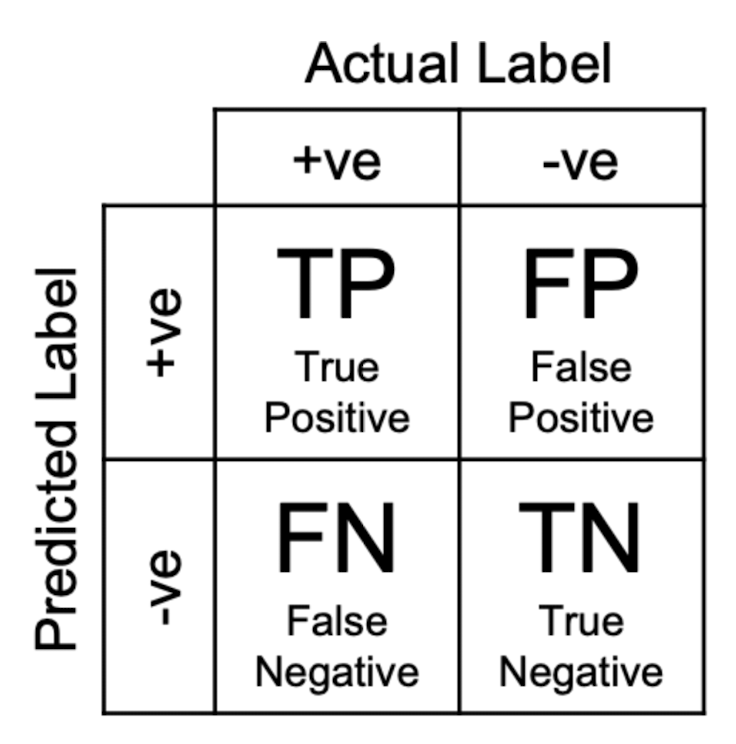
\includegraphics[scale=0.2]{confusion-matrix}

\begin{itemize}
    \item Accuracy = $\frac{TP + TN}{TP + FN + FP + TN}$
    \item \keyword{Precision}{$\frac{TP}{TP + FP}$} \keyword{Recall}{$\frac{TP}{TP + FN}$}
    \item Type I Error: FP Type II Error: FN
    \item FP Rate = $\frac{FP}{FP + TN}$ TP Rate = $\frac{TP}{TP + FN}$
\end{itemize}

\subsection{Pruning}

\begin{itemize}
    \item Motivation: DT overfits to training set, but performs poorly on test set
    \item Occam's Razor: Simple hypothesis preferred
    \item \keyword{Pruning}{Ignores outliers, which reduces overfitting}
    \begin{itemize}
        \item E.g. Min-sample, Max-depth
    \end{itemize}
\end{itemize}

\section{06. Linear Regression}

\subsubsection{Notation}

\begin{itemize}
    \item $m$ = Number of training examples
    \item $n$ = Number of features
    \item $x_j ^{(i)}$ = Input feature $j$ of $i$th training example
    \item $y$ = Output variables
\end{itemize}

\subsubsection{Hypothesis}

\[h_w (x): w_0 + w_1 x\]

\subsubsection{Cost Function (Square Error Function)}

\[J(w_0, w_1) = \frac{1}{2m} \sum_{i = 1}^{m} (h_w(x^{(i)}) - y^{(i)})^2\]

\begin{itemize}
    \item Goal: Minimize cost function. Thus, hypothesis is close to training samples
    \item Why squared error? Convenience, since we need to differentiate later
\end{itemize}

\subsection{Gradient Descent}

\begin{itemize}
    \item Start at some $(w_0, w_1)$. Pick nearby point that reduces $J(w_0, w_1)$.
    \item Algorithm: Repeat until convergence:
\end{itemize}

\[w_j := w_j - \alpha \frac{dJ(w_0, w_1, ...)}{dw_j}\]

\begin{itemize}
    \item All updates done at end
    \item How to do $\frac{dJ(w_0, w_1)}{dw_j}$? Partial derivative: Hold everything else constant
    \begin{itemize}
        \item $\frac{dJ(w_0, w_1)}{dw_j} = \frac{d}{dw_j} (\frac{1}{2m} \sum_{i = 1}^{m} (w_0 + w_1 x^{(i)} - y^{(i)})^2)$
        \item $\frac{dJ(w_0, w_1)}{dw_0} = \frac{1}{m} \sum_{i = 1}^{m} (w_0 + w_1 x^{(i)} - y^{(i)})$ (Note: Chain rule)
        \item $\frac{dJ(w_0, w_1)}{dw_1} = \frac{1}{m} \sum_{i = 1}^{m} (w_0 + w_1 x^{(i)} - y^{(i)}) x^{(i)}$
    \end{itemize}
    \item Time complexity: $O(kmn)$ where $k$ is number of iterations
\end{itemize}

\subsubsection{Learning Rate}

\begin{itemize}
    \item If $\alpha$ too small, then descent is too slow. If $\alpha$ too big, then might overshoot.
    \item Given constant $\alpha$, descent will grow smaller as we approach minimum
\end{itemize}

\subsubsection{Variants of Gradient Descent}

\begin{itemize}
    \item Batch gradient descent: Consider all training examples when updating
    \item Stoichastic gradient descent: Consider 1 random data point at a time (Cheaper and more randomness)
    \item Mini-batch gradient descent
\end{itemize}

\subsubsection{Using Matrices}

\begin{itemize}
    \item Given: $w = 
    \begin{pmatrix}
        w_0\\
        \vdots\\
        w_n
    \end{pmatrix}$ and $x =
    \begin{pmatrix}
        x_0\\
        \vdots\\
        x_n
    \end{pmatrix} = 
    \begin{pmatrix}
        1\\
        \vdots\\
        x_n
    \end{pmatrix}$
    \item $h_w(x): w^T x$
\end{itemize}

\subsubsection{Feature Scaling}

\begin{itemize}
    \item Motivation: Gradient descent does not work well if features have different scales
    \item \keyword{Mean Normalization}{$x_i \leftarrow \frac{x_i - \mu_i}{\sigma_i}$}
\end{itemize}

\subsection{Normal Equation}

\[w = (X^T X)^{-1} X^T Y\]

\begin{itemize}
    \item No need to choose $\alpha$ and feature scaling
    \item $X^T X$ needs to be invertible
    \item Time complexity: $O(n^3)$. Slow if $n$ is big
\end{itemize}

\section{07. Logistic Regression}

\end{multicols*}
\end{document}
